%
%  analysis_report
%
%  Created by Sam Cook on 2012-11-06.
%  Copyright (c) 2012 . All rights reserved.
%
\documentclass[]{article}

% Setup for fullpage use
\usepackage{fullpage}

% More symbols
\usepackage{amsmath}

% Allow merged rows/colums in tables
\usepackage{multirow}

% Package for including code in the document
\usepackage{listings}
% make sure that code listings wrap to the page reasonably nicely
% gobble removes first 4 characters, allows indentation for source readability
\lstset{breakindent=40pt, breaklines=true, gobble=4, captionpos=b}
% Apparently preloading lstlangauages speeds things up
\lstloadlanguages{C,C++}

% If you want to generate a toc for each chapter (use with book)
\usepackage{minitoc}

% This is now the recommended way for checking for PDFLaTeX:
\usepackage{ifpdf}

\ifpdf
\usepackage[pdftex]{graphicx}
\else
\usepackage{graphicx}
\fi

% useful commands for setting nth's (e.g. 5th) and alt versions (e.g. 2nd)
\newcommand{\nth}[1]{$#1^\text{th}$}
\newcommand{\nthTwo}[2]{$#1^\text{#2}$}
% quick macro for µs
\newcommand{\ms}{$~\mu$s}

\title{MuSIC 5 Analysis Report}
\author{Sam Cook}

\date{2012-11-06}

\begin{document}

\ifpdf
\DeclareGraphicsExtensions{.pdf, .jpg, .tif}
\else
\DeclareGraphicsExtensions{.eps, .jpg}
\fi

\maketitle


\begin{abstract}
	The \nth{5} MuSIC beam-time (\nth{18} to the \nthTwo{22}{nd} June 2012) was intended to test the momentum distribution of the muons beam. Here we will discuss the strategy employed to analyse the data and the problems encountered.
\end{abstract}

\section{Introduction} % (fold)
\label{sec:introduction}
The analysis of the \nth{5}~MuSIC beam time splits into 5~logical sub-algorithms called here: `Run Data' (Section~\ref{sec:run_data}), `Simulated Data' (Section~\ref{sec:simulated_data}), `Acceptance' (Section~\ref{sec:acceptance}), `Fitting and Integration' (Section~\ref{sec:fitting_and_integration}) and `Muon Yield' (Section~\ref{sec:muon_yield}). The `Run' and `Simulated Data' algorithms cover the processing of the initial data to such a point as they can be treated identically. The `Acceptance' section covers the calculation of the detector acceptance based on simulated data. The `Fitting and Integration' and `Muon Yield' sections cover the final stages of the algorithm in calculating the number of muon decays and ultimately the muon yield of the run. The overall flow can be seen in Figure~\ref{fig:analysis_flow_diagrm}. A brief overview of the experimental set up is given in section~\ref{sec:experimental_set_up}.

\begin{figure}[htbp]
	\centering
		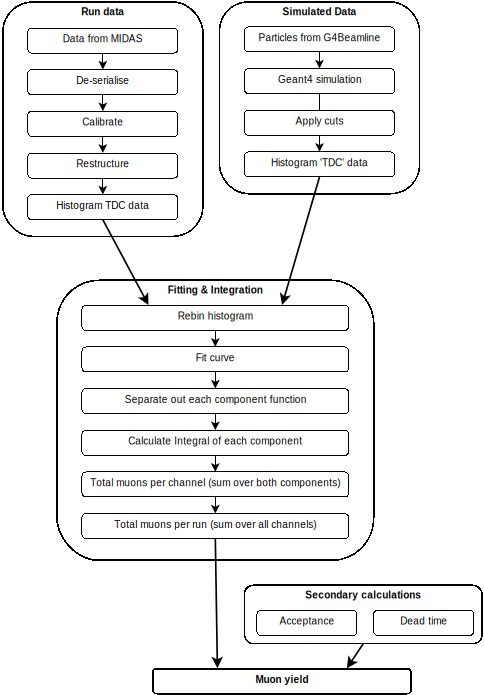
\includegraphics[height=0.49\textheight]{image/Analysis_flow_diagram.png}
	\caption{Flow diagram of the analysis' logic}
	\label{fig:analysis_flow_diagrm}
\end{figure}
% section introduction (end)
%%%%%%%%%%%%%%%%%%%%%%%%%%%%%%%%%%%%%%%%%%%%%%%%%%%%%%%%%%%%%%%%%%%%%%%%%%%%%%
\section{Experimental Set Up} % (fold)
\label{sec:experimental_set_up}
To measure the momentum distribution of the muon beam two separate problems had to be solved: firstly how to count the muons produced and secondly how to determine their momentum. The first problem is addressed by looking for muon decays through timing data whilst the second is dealt with by using degraders and a thin stopping target to select specific momentums. 

\subsection{Detector} % (fold)
\label{sub:detector}
The detector consisted of an aluminium degrader who's thickness could be varied to select different momentum ranges, a thin (1~mm) upstream counter and a thicker (3.5~mm) downstream counter on either side of a 0.5~mm copper stopping target. A schematic of the detector can be seen in figure~\ref{fig:setup}. Based on simulation (section~\ref{sec:simulated_data}) we can predict the mean momentum of muons that decay for different degrader thicknesses, the momentum distributions can be seen in figure~\ref{fig:stopped_muon_mom} with the mean momentums given in 
\begin{figure}[htbp]
	\centering
		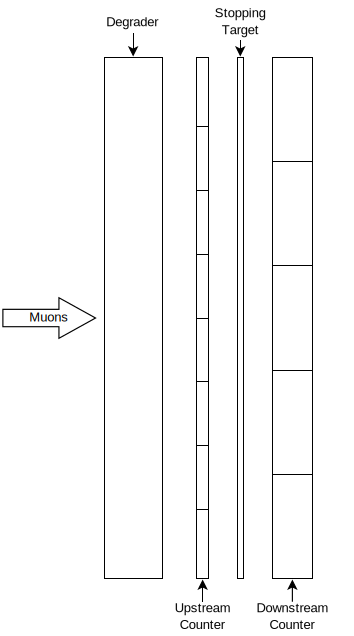
\includegraphics[scale=0.5]{image/Detector_setup.png}
	\caption{Experimental set up of the detector for MuSIC~5 (not to scale)}
	\label{fig:setup}
\end{figure}  
\begin{figure}[htbp]
	\centering
		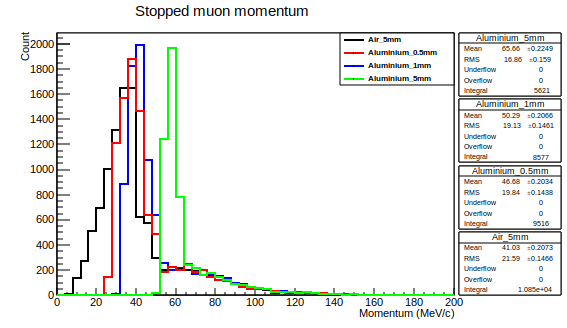
\includegraphics[width=\textwidth]{image/stopped_muon_momentum.png}
	\caption{Simulated momentum distributions for muons decaying between the up and downstream counters. 900~M initial protons were simulated with a range of aluminium degrader thicknesses.}
	\label{fig:stopped_muon_mom}
\end{figure}
\begin{table}
	\begin{center}
	\begin{tabular}{r|r@{ $\pm$ }l|r@{ $\pm$ }l} % r@{ $\pm$ }l should align on \pm
		Degrader (mm) & \multicolumn{2}{|c|}{Mean (MeV/c)} & \multicolumn{2}{|c}{RMS (MeV/c)}\\
		\hline
		Air 5.0       & 41.03 & 0.21 & 21.59 & 0.15 \\
		Aluminium 0.5 & 46.68 & 0.20 & 19.84 & 0.14 \\
		Aluminium 1.0 & 50.29 & 0.21 & 19.13 & 0.15 \\
		Aluminium 5.0 & 65.66 & 0.22 & 16.86 & 0.16 \\
	\end{tabular}
	\end{center}
	\caption{Simulated mean momentums for decaying muons. 900~M initial protons}
	\label{label}
\end{table}
The counters used are mylar wrapped scintillators with read-out performed by MPPCs mounted on either end of a wave length shifting fibre bounded along the long axis of the scintillator. The signals from each pair of MPPCs are combined and amplified before being passed to the data acquisition system (DAQ) for processing.

% subsection detector (end)
\subsection{Data Acquisition} % (fold)
\label{sub:data_acquisition}
The Data Acquisition (DAQ) took two measurements: the time at which signals arrived from the MPPC and the size of those signals. The timing measurements are of the primary concern for this analysis. The DAQ itself had 3 distinct stages: discrimination, trigger formation and readout.

MPPCs are inherently noisy devices and discrimination is required to separate signal due to scintillation events from the MPPC's noise; this was done by setting a voltage threshold which a signal had to exceed in order to be considered. Two thresholds were used: a lower one for the upstream counters and a higher one for those further downstream. The lower threshold for the, thinner, upstream counters enabled better detection of minimally ionising muons whilst the higher downstream threshold enabled better detection of the electrons produced by muonic decay. 

Once suitable signals had been discriminated for a trigger was created based on the signature of muonic decay. This was done by looking for anti-coincidence between the up and downstream counters. This was done on the assumption that a muon that doesn't decay in the detector region will be seen in both counters within a very small window of time (<50~ns). The only other constraint on the formation of a trigger was that the system wasn't busy in which case the trigger couldn't be accepted.

The trigger, once formed, signalled the start of readout there were two primary modules for readout a Multi-hit Time to Digital Converter (MTDC) which is the primary concern for this analysis and an Charge to Digital Converter (QDC). The MTDC recorded all suitable signals received at either the up or downstream counters in a 20\ms{} window after the trigger. Using a MTDC ensured that even if some beam remnant or dark event created a signal then the real signal would also be recorded and determined with background removal. The channel assignment used for the MTDC can be seen in table~\ref{tab:mtdc_ch}. To increase the accuracy of the MTDC the trigger time is recorded on a seperate channel called `TDC0'.
\begin{table}
	\begin{center}
	\begin{tabular}{c|c|c}
		Channel & Signal & Notes\\
		\hline
		0  & TDC0 & Time at which the trigger was formed \\
		\hline
		1  & U1   & \multirow{8}{*}{Upstream Counter}\\
		2  & U2   & \\
		3  & U3   & \\
		4  & U4   & \\
		5  & U5   & \\
		6  & U6   & \\
		7  & U7   & \\
		8  & U8   & \\
		\hline
		9  & D1   & \multirow{5}{*}{Downstream counter}\\
		10 & D2   & \\
		11 & D3   & \\
		12 & D4   & \\
		13 & D5   & \\
		\hline
		14 & Ge1  & \multirow{2}{*}{Germanium not used in this analysis}\\
		15 & Ge2  & \\
	\end{tabular}
	\end{center}
	\caption{Channel assignment for the MTDC. QDC channel assignment follows the same scheme but has no entry for channel 0 (as TDC 0 will be one of the upstream counters by design).}
	\label{tab:mtdc_ch}
\end{table}

A scaler was also used to continuously record various other diagnostics (see table~\ref{tab:scaler_chs}) for the experiment. The scaler was polled regularly throughout data taking. Some of these diagnostics are used as verification of the data (for example: using the ratio of triggers to potential triggers to estimate the dead time of the system).
\begin{table}
	\centering
	\begin{tabular}{c|c|l}
		Channel & Signal & Notes\\
		\hline
		0 & SEC & Measure of the proton current\\
		1 & Trigger & number of t0's\\
		2 & U and $\overline{\text{D}}$ & count of potential triggers\\
		3 & U & Upstream only\\
		4 & D & Downstream only\\
		5 & Scint & -\\
		6 & unused & -\\
		7 & clk & Record of time passed\\
	\end{tabular}
	\caption{Table of scaler channels and their designation}
	\label{tab:scaler_chs}
\end{table}

% subsection data_acquisition (end)
% section experimental_set_up (end)
%%%%%%%%%%%%%%%%%%%%%%%%%%%%%%%%%%%%%%%%%%%%%%%%%%%%%%%%%%%%%%%%%%%%%%%%%%%%%%
\section{Run Data} % (fold)
\label{sec:run_data}
As figure~\ref{fig:analysis_flow_diagrm} shows there are 5 main stages in preparing the real data for analysis (receipt of the data from MIDAS, de-serialisation, calibration, restructuring and histogramming). These will will be explained in more detail in the following sub-sections but the general process will be discussed here. The first stage is the receipt of data from the DAQ via MIDAS, this creates files of raw data which has to be (in some cases) de-serialised in the next stage before having calibration applied to it. The final stages are to restructure the data according to channel and then create histograms of the TDC values ready for analysis. 

These processes are split across 4 programs: MIDAS; mu\_analysis and mid2root\_converter (which act on .root and .mid MIDAS files respectively); and finally tdc\_file.py which is a python script for creating the TDC histograms.

\subsection{Data from MIDAS} % (fold)
\label{sub:data_from_midas}
MIDAS is `a general purpose data acquisition system for small and medium scale experiments' \ref{MIDAS REF PLEASE!} and is the primary interface to the DAQ. As discussed in section~\ref{sub:data_acquisition} there were two asynchronous systems in the DAQ to be read out: the trigger and the scaler systems (the QDC and MTDC making up the trigger; the scaler on its own). MIDAS stores the raw data from the VME crate (MTDC, QDC and Scaler) in their respective structures either as binary xml (.mid files) or within binary root files (.root).

The structure received from MIDAS consisted of a tree for each VME module used. Each tree consisted of two integer branches: `nX' and `X[nX]' where `X' was the name of the module (i.e `TDC', used for the MTDC, or `QDC').
% subsubsection data_from_midas (end)
\subsection{De-Serialisation} % (fold)
\label{sub:de_serialisation}
The first problem with the raw data from MIDAS is that the information from the MTDC is serialised and mangled with the channel number, i.e. the data from each channel is tagged with the channel number and not read out in a predictable manner. The same is true of the QDC data but not the scaler information. Below are brief summaries of the algorithms used to de-serialise the MTDC data, for full listings see appendix~\ref{app:deserialisation}.
%
\begin{center}
\begin{lstlisting} [caption={Pseudo-code demonstrating the de-serialisation of the raw MTDC data from MIDAS (for a CAEN V1290N). \textbf{NB} `$\&$' is a bit-wise AND; `$>>$'is a right bit-shift and `$==$' is a logical equals.}, label={lst:tdc_deserialisation}, float=htbp, language=C++]
    tdc_value      =  raw_val & 0x001f ffff
    tdc_channel    = (raw_val & 0x03e0 0000) >> 21
    tdc_valid_read = (raw_val & 0xf800 0000) == 0x0
\end{lstlisting}
\end{center}
% subsection de_serialisation (end)
\subsection{Calibration} % (fold)
\label{sub:calibration}
The MTDC has a stated least significant bit resolution of $\sim$25~ps with 21 bit of data, this gives a maximum range of 52\ms{}. Conversion from the stored value to real, trigger aligned, time is done using the formula:
\begin{align}\label{equ:tdc_calibration}
	t' = 1.025\times\frac{t - TDC0}{40}
\end{align}
where $t'$ is the calibrated time, $t$ is the MTDC value and $TDC0$ is the trigger time. The factor, $1.025$, is derived by feeding a known clock into to the MTDC whilst the factor $40$ converts from ps to ns.
% subsection calibration (end)
\subsection{Restructure} % (fold)
\label{sub:restructure}
In order to be more easily manipulated the MIDAS data has to be restructured. The initial format is a simple structure of one branch for each module (i.e. one for MTDC one for the QDC and a final one for errors). A second tree is used to store the scaler values. 

In the restructured file each channel is a branch of a tree with the following leaves: QDC, TDC0, nHITS, TDC[nHITS]. The QDC value is self-explanatory, TDC0 is the trigger time, nHITS is the number of entries recorded by the MTDC for that channel and TDC is an array of these values. The error data is ignored as is the scaler tree as these can be read from the original file if needed as neither require de-serialisation or calibration.
% subsection restructure (end)
\subsection{Histogramming} % (fold)
\label{sub:Histogramming}
Once the data has been restructured it is trivial to create a histogram of the TDC data for each channel which forms the basis of the later analysis.
% subsection histogramming (end)
% section run_data (end)
%%%%%%%%%%%%%%%%%%%%%%%%%%%%%%%%%%%%%%%%%%%%%%%%%%%%%%%%%%%%%%%%%%%%%%%%%%%%%%
\section{Simulated Data} % (fold)
\label{sec:simulated_data}

% section simulated_data (end)
%%%%%%%%%%%%%%%%%%%%%%%%%%%%%%%%%%%%%%%%%%%%%%%%%%%%%%%%%%%%%%%%%%%%%%%%%%%%%%
\section{Acceptance} % (fold)
\label{sec:acceptance}

% section acceptance (end)
%%%%%%%%%%%%%%%%%%%%%%%%%%%%%%%%%%%%%%%%%%%%%%%%%%%%%%%%%%%%%%%%%%%%%%%%%%%%%%
\section{Fitting And Integration} % (fold)
\label{sec:fitting_and_integration}

% section fitting_and_integration (end)
%%%%%%%%%%%%%%%%%%%%%%%%%%%%%%%%%%%%%%%%%%%%%%%%%%%%%%%%%%%%%%%%%%%%%%%%%%%%%%
\section{Muon Yield} % (fold)
\label{sec:muon_yield}

% section muon_yield (end)
%%%%%%%%%%%%%%%%%%%%%%%%%%%%%%%%%%%%%%%%%%%%%%%%%%%%%%%%%%%%%%%%%%%%%%%%%%%%%%
\appendix
\section{De-serialisation code} % (fold)
\label{app:deserialisation}

\begin{center}
	\begin{lstlisting}[caption={Functions used for de-serialising CAEN V1290N \ref{REF FOR THE DATA SHEET} MTDC  output, written in C++}, language=C++, float=htbp]
    inline int midus_file::get_tdc_val(const int index) const {
        unsigned int const tdc_data_mask = 0x01fffff;
        unsigned int const val = static_cast<unsigned int>(branches_m[tdc_i].data[index]);
        return static_cast<int>(val & tdc_data_mask);
    }
    
    inline int midus_file::get_tdc_ch(const int index) const {
        unsigned int const tdc_channel_mask = 0x03e00000;
        unsigned int const val = static_cast<unsigned int>(branches_m[tdc_i].data[index]);
        return static_cast<int>((val & tdc_channel_mask) >> 21);
    }
    
    inline bool midus_file::is_good_tdc_measure(const int index) const {
        unsigned int const tdc_data_type_mask = 0xf8000000;
        unsigned int const tdc_measurement    = 0x00000000;
        unsigned int const val = static_cast<unsigned int>(branches_m[tdc_i].data[index]);
        return ((val & tdc_data_type_mask) == tdc_measurement);
    }
	\end{lstlisting}
\end{center}

\begin{center}
	\begin{lstlisting}[caption={Functions used for de-serialising CAEN V792N \ref{REF FOR THE DATA SHEET} QDC, written in C++}, language=C++, float=htbp]
    inline int midus_file::get_qdc_val(int const index) const {
    	unsigned int const data_mask = 0x00000fff;
    	unsigned int const val = static_cast<unsigned int>(branches_m[qdc_i].data[index]);
    	return static_cast<int>(val & data_mask); 
    }
    
    inline int midus_file::get_qdc_ch(const int index) const {
        unsigned int const channel_mask = 0x001f0000;
        unsigned int const val = static_cast<unsigned int>( branches_m[qdc_i].data[index]);
        return static_cast<int>((val & channel_mask) >> 17);
    }
    
    inline bool midus_file::is_good_qdc_measure(const int index) const {
        unsigned int const underflow_mask = 0x00002000;
        unsigned int const overflow_mask  = 0x00001000;
        unsigned int const val = static_cast<unsigned int>(branches_m[tdc_i].data[index]);
        return !((underflow_mask & val) || (overflow_mask & val));
    }
	\end{lstlisting}

\end{center}

% section tdc_deserialisation (end)
\bibliographystyle{plain}
\bibliography{}
\end{document}
